% !TeX encoding = UTF-8
% !TeX spellcheck = pl_PL

% $Id:$

%Author: Wojciech Domski
%Szablon do ząłożeń projektowych, raportu i dokumentacji z steorwników robotów
%Wersja v.1.0.0
%


%% Konfiguracja:
\newcommand{\kurs}{Sterowniki robot\'{o}w}
\newcommand{\formakursu}{Projekt}

%odkomentuj właściwy typ projektu, a pozostałe zostaw zakomentowane
\newcommand{\doctype}{Za\l{}o\.{z}enia projektowe} %etap I
%\newcommand{\doctype}{Raport} %etap II
%\newcommand{\doctype}{Dokumentacja} %etap III

%wpisz nazwę projektu
\newcommand{\projectname}{Wykrywacz kradzieży}

%wpisz akronim projektu
\newcommand{\acronim}{WK}

%wpisz Imię i nazwisko oraz numer albumu
\newcommand{\osobaA}{Sylwester \textsc{Kozieja}, 235798}
%w przypadku projektu jednoosobowego usuń zawartość nowej komendy
\newcommand{\osobaB}{Paula \textsc{Langkafel}, 235373}

%wpisz termin w formie, jak poniżej dzień, parzystość, godzina
\newcommand{\termin}{\'sroda TN 13}

%wpisz imię i nazwisko prowadzącego
\newcommand{\prowadzacy}{mgr in\.{z}. Wojciech \textsc{Domski}}

\documentclass[10pt, a4paper]{article}

%Preambuła dokumentu

% linki w spisie tresci, bibliografi
\usepackage[bookmarks=true,bookmarksnumbered=false,unicode=true,pdftex=true, colorlinks,filecolor=black,linkcolor=black,urlcolor=black,citecolor=black]{hyperref}

%ustawienie rozmiaru papieru
\usepackage[a4paper, left=2.5cm, right=2.5cm, top=2.5cm, bottom=2.5cm, headsep=1.2cm]{geometry}

%rozmaite ustawienia pozwalające okreslić język

%NALEŻY wybrać jeden z pakietów
%\usepackage{polski} %przydatne podczas składania dokumentów w j. polskim
\usepackage[polish]{babel}  % pakiet lokalizujący dokument w języku polskim
%\usepackage[british]{babel}

\usepackage{indentfirst}	% polski styl pisania (np. rozpoczecie pierwszego akapitu
% pod nazwa rozdzialu od wciecia)
%\usepackage[OT4]{fontenc}
\usepackage[utf8]{inputenc} % w miejsce utf8 można wpisać latin2 bądź cp1250,
% w zależności od tego w jaki sposób kodowane są 
% polskie znaki diakrytyczne przy wprowadzaniu 
% z klawiatury.
%kodowanie znaków, zależne od systemu
\usepackage[T1]{fontenc} %poprawne składanie polskich czcionek

%OPEROWANIE NA OBRAZACH
\usepackage{graphicx}       % pakiet graficzny, umożliwiający m.in.
% import grafik w formacie eps
%\usepackage{epstopdf}		% pozwala na importowanie grafik w formacie eps
% przy użyciu pdflatex
\usepackage[update,prepend]{epstopdf}
\usepackage{rotating}       % pakiet umożliwiający obracanie rysunków
\usepackage{subfigure}      % pakiet umożliwiający tworzenie podrysunków
\usepackage{epic}           % pakiet umożliwiający rysowanie w środowisku latex
\usepackage{psfrag}         % pakiet umożliwiający podmianę łańcuchów znaków 
% w plikach eps
%\usepackage{curves}         % pakiet do wykreslania krzywych

%pakiety dodające dużo dodatkowych poleceń matematycznych
\usepackage{amsfonts}       % pakiet z rozmaitymi czcionkami matematycznymi
%\usepackage{amssymb}        % pakiet z rozmaitymi symbolami matematycznymi
\usepackage{amsmath}        % pakiet z rozmaitymi środowiskami matematycznymi

\usepackage{fp}             % pakiet z funkcjami operujacymi 
% na liczbach zmiennoprzecinkowych
\usepackage{calc}           % pakiet umożliwiający operacje arytmetyczne
% na tzw. licznikach (liczbach całkowitych)
\usepackage{leftidx}		% indeksy górne i dolne po lewej stronie

%definicje matematyczne
\providecommand{\abs}[1]{\lvert#1\rvert}
\providecommand{\norm}[1]{\lVert#1\rVert}

%pakiety wspomagające i poprawiające składanie tabel
\usepackage{supertabular}
\usepackage{array}
\usepackage{tabularx}
\usepackage{hhline}
\usepackage{longtable}		% wsparcie dla dlugich tabel
\usepackage{multicol}		% podzial strony na wiele kolumn

%pakiet do BibTex
\usepackage{cite}

\usepackage{url} %pakiet pozawalający na dodawanie adresów url w bibliografi

%pakiet wypisujący na marginesie etykiety równań i rysunków zdefiniowanych przez \label{}, chcąc wygenerować finalną wersję dokumentu wystarczy usunąć poniższą linię
%\usepackage{showlabels}

\usepackage{float}			% lepsza obsluga mechanizmow obiektow plywajacych
% wymuszenie wstawienia np. tabeli, obrazka w danym miejscu przez [H]

\usepackage{listings}       % pakiet dedykowany zrodlom programow
\usepackage{color}


\definecolor{dkgreen}{rgb}{0,0.6,0}
\definecolor{gray}{rgb}{0.5,0.5,0.5}
\definecolor{mauve}{rgb}{0.58,0,0.82}

\lstset{ %
	language=C,                % the language of the code
	basicstyle=\small,           % the size of the fonts that are used for the code
	numbers=left,                   % where to put the line-numbers
	numberstyle=\footnotesize\color{gray},  % the style that is used for the line-numbers
	stepnumber=1,                   % the step between two line-numbers. If it's 1, each line 
	% will be numbered
	numbersep=5pt,                  % how far the line-numbers are from the code
	backgroundcolor=\color{white},      % choose the background color. You must add \usepackage{color}
	showspaces=false,               % show spaces adding particular underscores
	showstringspaces=false,         % underline spaces within strings
	showtabs=false,                 % show tabs within strings adding particular underscores
	%frame=single,                   % adds a frame around the code
	rulecolor=\color{black},        % if not set, the frame-color may be changed on line-breaks within not-black text (e.g. comments (green here))
	tabsize=2,                      % sets default tabsize to 2 spaces
	captionpos=b,                   % sets the caption-position to bottom
	breaklines=true,                % sets automatic line breaking
	breakatwhitespace=false,        % sets if automatic breaks should only happen at whitespace
	%title=\lstname,                   % show the filename of files included with \lstinputlisting;
	% also try caption instead of title
	keywordstyle=\color{blue},          % keyword style
	commentstyle=\color{dkgreen},       % comment style
	stringstyle=\color{mauve},         % string literal style
	escapeinside={\%*}{*)},            % if you want to add LaTeX within your code
	morekeywords={*,...},              % if you want to add more keywords to the set
	deletekeywords={...}              % if you want to delete keywords from the given language
}

%polish signs in lst code
\lstset{literate=%
	{ą}{{\k{a}}}1
	{ć}{{\'c}}1
	{ę}{{\k{e}}}1
	{ł}{{\l}}1
	{ń}{{\'n}}1
	{ó}{{\'o}}1
	{ś}{{\'s}}1
	{ż}{{\.z}}1
	{ź}{{\'z}}1
	{Ą}{{\k{A}}}1
	{Ć}{{\'C}}1
	{Ę}{{\k{E}}}1
	{Ł}{{\L}}1
	{Ń}{{\'N}}1
	{Ó}{{\'O}}1
	{Ś}{{\'S}}1
	{Ż}{{\.Z}}1
	{Ź}{{\'Z}}1
}

\usepackage{verbatim}       % pakiet dedykowany rozmaitym wydrukom tekstowym
\usepackage{ifthen}         % pakiet umożliwiający tworzenie prostych programów
% (m.in. zawiera instrukcje powtórzeniowe 
% i warunkowe)
\usepackage{upquote}		%normal quotations marks ' and `

% deklaracje wymagane przez pakiet theorem automatycznie ladowany w przypadku
% klasy dokumentu article
%
\newtheorem{Dn}{Definicja}[section]     % deklaracja srodowiska definicja
\newtheorem{La}[Dn]{Lemat}                % deklaracja srodowiska lemat
\newtheorem{Tm}[Dn]{Twierdzenie}          % deklaracja srodowiska twierdzenie
\newtheorem{Rk}[Dn]{Spostrze{\.z}enie}  % deklaracja srodowiska spostrzezenie
\newtheorem{Am}[Dn]{Algorytm}           % deklaracja srodowiska algorytm
\newtheorem{As}[Dn]{Za{\l}o{\.z}enie}   % deklaracja srodowiska zalozenie
\newtheorem{Pn}[Dn]{Propozycja}           % deklaracja srodowiska propozycja
\newtheorem{Py}[Dn]{W{\l}asno{\'s}{\'c}}  % deklaracja srodowiska wlasnosc
\newtheorem{Cy}[Dn]{Wniosek}              % deklaracja srodowiska wniosek
\newtheorem{Ee}[Dn]{Przyk{\l}ad}        % deklaracja srodowiska przyklad
\newtheorem{Ex}{{\'C}wiczenie}          % deklaracja srodowiska cwiczenie

%helps to specify width of a column in table
%\begin{tabular}{|C{1cm}|c|c|c|c|c|c|c|c|c|c|}
%first column will have widht of 1cm
\newcolumntype{L}[1]{>{\raggedright\let\newline\\\arraybackslash\hspace{0pt}}m{#1}}
\newcolumntype{C}[1]{>{\centering\let\newline\\\arraybackslash\hspace{0pt}}m{#1}}
\newcolumntype{R}[1]{>{\raggedleft\let\newline\\\arraybackslash\hspace{0pt}}m{#1}}

\sloppy			%zawija bardzo długie linie

%\pagenumbering{gobble}% Remove page numbers (and reset to 1)
\usepackage{hyperref}	
\begin{document}

\def\tablename{Tabela}	%zmienienie nazwy tabel z Tablica na Tabela

\begin{titlepage}
	\begin{center}
		\textsc{\LARGE \formakursu}\\[1cm]		
		\textsc{\Large \kurs}\\[0.5cm]		
		\rule{\textwidth}{0.08cm}\\[0.4cm]
		{\huge \bfseries \doctype}\\[1cm]
		{\huge \bfseries \projectname}\\[0.5cm]
		{\huge \bfseries \acronim}\\[0.4cm]
		\rule{\textwidth}{0.08cm}\\[1cm]
		
		\begin{flushright} \large
		\emph{Skład grupy:}\\
		\osobaA\\
		\osobaB\\[0.4cm]
		
		\emph{Termin: }\termin\\[0.4cm]

		\emph{Prowadzący:} \\
		\prowadzacy \\
		
		\end{flushright}
		
		\vfill
		
		{\large \today}
	\end{center}	
\end{titlepage}

\newpage
\tableofcontents
\newpage

%Obecne we wszystkich dokumentach
\section{Opis projektu}
\label{sec:OpisProjektu}
%Jak rozumieć moduły
Celem projektu jest stworzenie urządzenia, które poprzez komunikację z akcelerometrem wykrywa niepożądany ruch. Użytkownik będzie miał możliwość wybrania sposobu otrzymywania komunikatów. Jednym z założeń projektu jest wybór opcjonalnego interfejsu audio. Urządzenia ma zawierać menu dające możliwość podstawowej konfiguracji, takiej jak załączenie alarmu i wybór sposobu komunikowania się oraz ustawianie poziomu załączania alarmu. Dodatkową opcją jest wizualizowanie poziomu rejestrowanych przyspieszeń. \\ 
Na zakres prac składa się oprogramowanie zewnętrznej pamięci Flash , skonfigurowanie akcelerometru, a także realizacja komunikacji z interfejsami.

\section{Konfiguracja mikrokontrolera}
\begin{figure}[H]
\centering
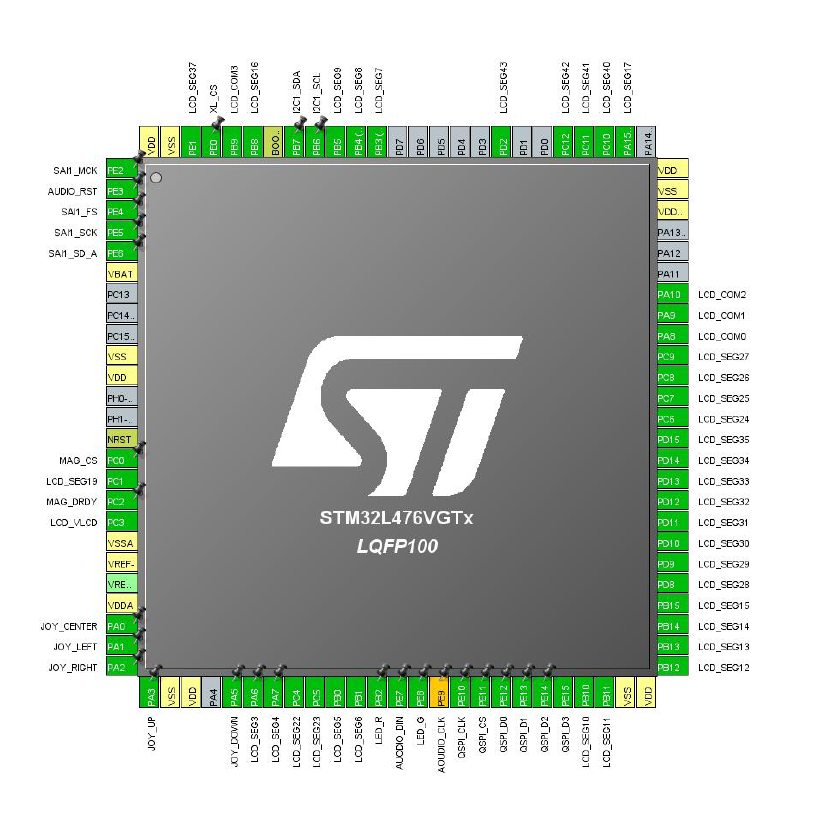
\includegraphics[width=13cm]{figures/cub.png}
\caption{Konfiguracja wyjść mikrokontrolera w programie STM32CubeMx}
\end{figure}
\newpage

\begin{figure}[H]
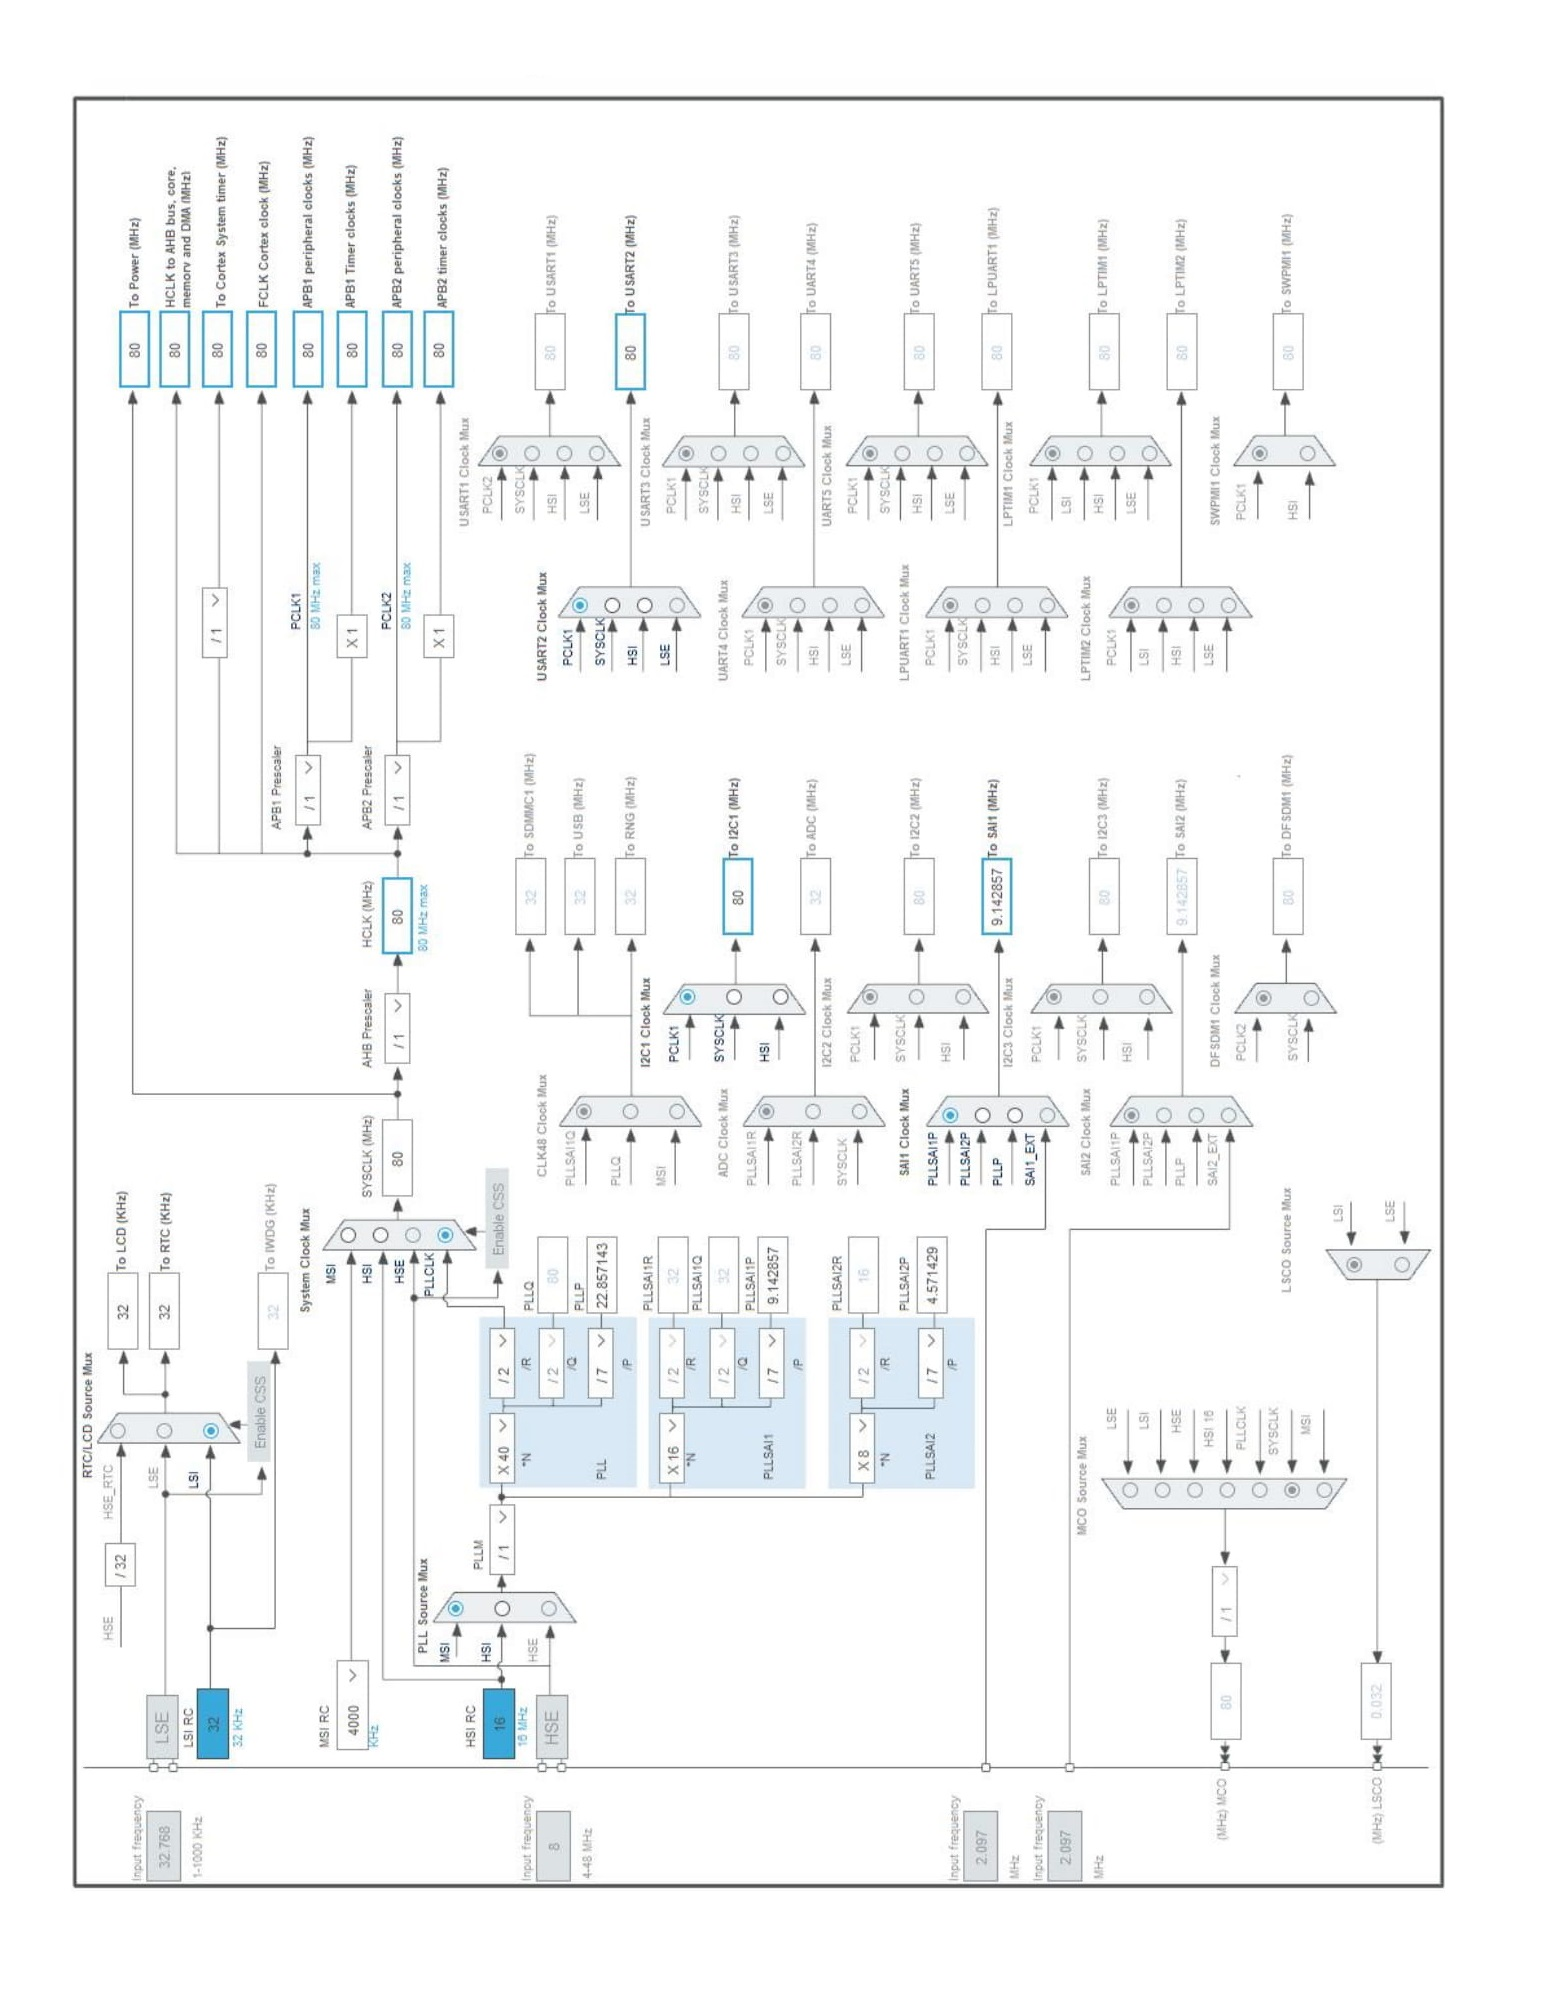
\includegraphics[width=17cm]{figures/zeg.jpg}
\caption{Konfiguracja zegarów mikrokontrolera}
\end{figure}

\subsection{Konfiguracja pinów mikrokontrolera}
\begin{table}[H]
\centering
\begin{tabular}{|l|L{2cm}|L{6cm}|L{4cm}|}
\hline
\textbf{Numer pinu} & \textbf{Pin} & \textbf{Tryb pracy} & \textbf{Funkcja/ etykieta} \\ \hline \hline
1&		PE2&		SAI1\_MCLK\_A	&	SAI1\_MCK	\\
2&		PE3	&	GPIO\_Output		&	AUDIO\_RST\\
3&		PE4	&	SAI1\_FS\_A			&	SAI1\_FS\\
4&		PE5	&	SAI1\_SCK\_A		&	SAI1\_SCK\\
5&		PE6	&	SAI1\_SD\_A	& \\
15&		PC0	&	GPIO\_Output		&	MAG\_CS\\
16&		PC1	&	LCD\_SEG19	& \\
17&		PC2	&	GPIO\_Input	&		MAG\_DRDY\\
18	&	PC3	&	LCD\_VLCD	& \\
23&		PA0	&	GPIO\_EXTI0	&		JOY\_CENTER\\
24	&	PA1	&	GPIO\_EXTI1	&		JOY\_LEFT\\
25&		PA2	&	GPIO\_EXTI2	&		JOY\_RIGHT\\
26	&	PA3	&	GPIO\_EXTI3	&		JOY\_UP\\
30&		PA5	&	GPIO\_EXTI5	&		JOY\_DOWN\\
31	&	PA6	&	LCD\_SEG3	&	\\
32	&	PA7	&	LCD\_SEG4	&	\\
33	&	PC4	&	LCD\_SEG22	&	\\
34	&	PC5	&	LCD\_SEG23	&	\\
35	&	PB0	&	LCD\_SEG5	&	\\
36	&	PB1	&	LCD\_SEG6	&	\\
37	&	PB2	&	GPIO\_Output	&		LED\_R\\
38	&	PE7	&	SAI1\_SD\_B	&		AUODIO\_DIN\\
39	&	PE8	&	GPIO\_Output	&		LED\_G\\
40	&	PE9*&	SAI1\_FS\_B	&		AOUDIO\_CLK\\
41	&	PE10&	QUADSPI\_CLK	&		QSPI\_CLK\\
42	&	PE11&	QUADSPI\_NCS	&		QSPI\_CS\\
43	&	PE12&	QUADSPI\_BK1\_IO0&		QSPI\_D0\\
44	&	PE13&	QUADSPI\_BK1\_IO1	&	QSPI\_D1\\
45	&	PE14&	QUADSPI\_BK1\_IO2	&	QSPI\_D2\\
46	&	PE15&	QUADSPI\_BK1\_IO3	&	QSPI\_D3\\
47	&	PB10&	LCD\_SEG10	&\\
48	&	PB11&	LCD\_SEG11	&\\
51	&	PB12&	LCD\_SEG12	&\\
52	&	PB13&	LCD\_SEG13	&\\
53	&	PB14&	LCD\_SEG14	&\\
54 &	PB15&	LCD\_SEG15	&\\
55	&	PD8	&	LCD\_SEG28	&\\
56	&	PD9	&	LCD\_SEG29	&\\
57	&	PD10&	LCD\_SEG30	& \\
58	&	PD11&	LCD\_SEG31	&\\
59	&	PD12&	LCD\_SEG32	&\\
60	&	PD13&	LCD\_SEG33	&\\
61	&	PD14&	LCD\_SEG34	&\\
62	&	PD15&	LCD\_SEG35	&\\
63	&	PC6	&	LCD\_SEG24	&\\
64	&	PC7	&	LCD\_SEG25	&\\
65	&	PC8	&	LCD\_SEG26	&\\
66	&	PC9	&	LCD\_SEG27	&\\
67	&	PA8	&	LCD\_COM0	&\\
68	&	PA9	&	LCD\_COM1	&\\
69	&	PA10&	LCD\_COM2	&\\
77	&	PA15 &	(JTDI) LCD\_SEG17&	\\
78	&	PC10&	LCD\_SEG40	&\\ \hline

\end{tabular}
\caption{Konfiguracja pinów mikrokontrolera}
\end{table}

\begin{table}[H]
\centering
\begin{tabular}{|l|L{2cm}|L{6cm}|L{4cm}|}
\hline
\textbf{Numer pinu} & \textbf{Pin} & \textbf{Tryb pracy} & \textbf{Funkcja/ etykieta} \\ \hline \hline
79	&	PC11&	LCD\_SEG41	&\\
80	&	PC12&	LCD\_SEG42	&\\
83	&	PD2	&	LCD\_SEG43	&\\
89	&	PB3 &	(JTDO-TRACESWO)	LCD\_SEG7&\\	
90	&	PB4 &	(NJTRST)LCD\_SEG8	&\\
91	&	PB5	&	LCD\_SEG9	&\\
92	&	PB6	&	I2C1\_SCL	&\\
93	&	PB7	&	I2C1\_SDA	&\\
95	&	PB8	&	LCD\_SEG16	&\\
96	&	PB9	&	LCD\_COM3	&\\
97	&	PE0	&	GPIO\_Output	&		XL\_CS\\
98	&	PE1	&	LCD\_SEG37	&\\ \hline
\end{tabular}
\caption{Konfiguracja pinów mikrokontrolera}
\end{table}

%\subsection{Konfiguracja peryferiów}
%\begin{table}[H]
%\centering
%\begin{tabular}{|l|l|l|l|}
%\hline
%Peryferia	&MODES&	FUNCTIONS	&PINS\\ \hline
%I2C1&	I2C&	I2C1\_SCL&	PB6\\
%I2C1&	I2C&	I2C1\_SDA&	PB7\\
%LCD&	1/4 Duty Cycle&	LCD\_VLCD&	PC3\\
%LCD&	1/4 Duty Cycle&	LCD\_COM0&	PA8\\
%LCD&	1/4 Duty Cycle&	LCD\_COM1&	PA9\\
%LCD&	1/4 Duty Cycle&	LCD\_COM2&	PA10\\
%LCD&	1/4 Duty Cycle&	LCD\_COM3&	PB9\\
%LCD&	SEG3&	LCD\_SEG3&	PA6\\
%LCD&	SEG4&	LCD\_SEG4&	PA7\\
%LCD&	SEG5&	LCD\_SEG5&	PB0\\
%LCD&	SEG6&	LCD\_SEG6&	PB1\\
%LCD&	SEG7&	LCD\_SEG7&	PB3 (JTDO-TRACESWO)\\
%LCD&	SEG8&	LCD\_SEG8&	PB4 (NJTRST)\\
%LCD&	SEG9&	LCD\_SEG9&	PB5\\
%LCD&	SEG10&	LCD\_SEG10&	PB10\\
%LCD&	SEG11&	LCD\_SEG11&	PB11\\
%LCD&	SEG12&	LCD\_SEG12&	PB1\\
%LCD&	SEG13&	LCD\_SEG13&	PB13\\
%LCD&	SEG14&	LCD\_SEG14&	PB14\\
%LCD&	SEG15&	LCD\_SEG15&	PB15\\
%LCD&	SEG16&	LCD\_SEG16&	PB8\\
%LCD&	SEG17&	LCD\_SEG17&	PA15 (JTDI)\\
%LCD&	SEG19&	LCD\_SEG19&	PC1\\
%LCD&	SEG22&	LCD\_SEG22&	PC4\\
%LCD&	SEG23&	LCD\_SEG23&	PC5\\
%LCD&	SEG24&	LCD\_SEG24&	PC6\\
%LCD&	SEG25&	LCD\_SEG25&	PC7\\
%LCD&	SEG26&	LCD\_SEG26&	PC8\\
%LCD&	SEG27&	LCD\_SEG27&	PC9\\
%LCD&	SEG28&	LCD\_SEG28&	PD8\\
%LCD&	SEG29&	LCD\_SEG29&	PD9\\
%LCD&	SEG30&	LCD\_SEG30&	PD10\\
%LCD&	SEG31&	LCD\_SEG31&	PD11\\
%LCD&	SEG32&	LCD\_SEG32&	PD12\\
%LCD&	SEG33&	LCD\_SEG33&	PD13\\
%LCD&	SEG34&	LCD\_SEG34&	PD14\\
%LCD&	SEG35&	LCD\_SEG35&	PD15\\
%LCD&	SEG37&	LCD\_SEG37&	PE1\\
%LCD&	SEG40&	LCD\_SEG40&	PC10\\
%LCD&	SEG41&	LCD\_SEG41&	PC11\\
%LCD&	SEG42&	LCD\_SEG42&	PC12\\
%LCD&	SEG43&	LCD\_SEG43&	PD2\\
%QUADSPI&	Quad SPI Line&	QUADSPI\_BK1\_IO0&	PE12\\
%QUADSPI&	Quad SPI Line&	QUADSPI\_BK1\_IO1&	PE13\\
%QUADSPI&	Quad SPI Line&	QUADSPI\_BK1\_IO2&	PE14\\
%QUADSPI&	Quad SPI Line&	QUADSPI\_BK1\_IO3&	PE15\\
%QUADSPI&	Quad SPI Line&	QUADSPI\_NCS&	PE11\\
%QUADSPI&	Quad SPI Line&	QUADSPI\_CLK&	PE10\\
%RTC&	Activate RTC Clock Source&	RTC\_VS\_RTC\_Activate&	VP\_RTC\_VS\_RTC\_Activate\\
%RTC&	RTC Enabled&	RTC\_VS\_RTC\_Calendar	&VP\_RTC\_VS\_RTC\_Calendar\\
%SAI1:SAI A&	Master with Master Clock Out&	SAI1\_SD\_A&	PE6\\
%SAI1:SAI A&	Master with Master Clock Out&	SAI1\_SCK\_A&	PE5\\
%SAI1:SAI A&	Master with Master Clock Out&	SAI1\_FS\_A&	PE4\\
%SAI1:SAI A&	Master with Master Clock Out&	SAI1\_MCLK\_A	&PE2\\
%SAI1:SAI B&	SPDIF TX Transmitter (IEC60958)	&SAI1\_SD\_B&
%	PE7\\
%SYS	&	SysTick	SYS\_VS\_Systick&	VP\_SYS\_VS\_Systick& \\
%\hline
%\end{tabular}
%\caption{Tabela z peryferiami}
%\end{table}

%\begin{enumerate}
\subsection{QUADSPI}
Interfejs użyty do obsługi pamięci Flash zapewniający dużą przepustowość dzięki czterem liniom danych (PE12:15) oraz dwóm liniom sterującym (PE10 i PE11).
\begin{table}[H]
\centering
\begin{tabular}{|l|c|}
\hline
\textbf{Parametr} & Wartość \\
\hline
\hline
\textbf{Clock Prescaler} & 255\\ \hline
\textbf{Fifo Threshold} & 1\\ \hline
\textbf{Sample Shifting} & No Sample Shifting \\ \hline
\textbf{Flash Size} & 1 \\ \hline
\textbf{Chip Select High Time} & 1 Cycle \\ \hline
\textbf{Clock Mode} & Low \\ \hline
\end{tabular}
\end{table}


\subsection{LCD}
Interfejs wyświetlacza umożliwiający komunikację z urządzeniem poprzez zaprojektowane menu. Korzysta z dużej ilości pinów, które opisane są na rysunku z konfiguracją. Ustawienia standardowe,parametr Duty Selection ustawiony na 1/4.

\begin{table}[H]
\centering
\begin{tabular}{|l|c|}
\hline
\textbf{Parametr} & Wartość \\
\hline
\hline
\textbf{Clock Prescaler} & 1 \\ \hline
\textbf{Clock Divider} & 16\\ \hline
\textbf{Duty Selection} & 1/4\\ \hline
\textbf{Bias Selector} & 1/4\\ \hline
\textbf{Multiplex mode} & Disable\\ \hline
\textbf{Voltage Source Selection} & Internal\\ \hline
\textbf{Contrast Control} & 2.60V\\ \hline
\textbf{Dead Time Duration} & No dead Time\\ \hline
\textbf{High Drive} & Disable\\ \hline
\textbf{Pulse ON Duration} & 0 pulse\\ \hline
\textbf{Blink Mode} & Disabled\\ \hline
\textbf{Blink Frequency} & fLCD/8\\ \hline

\end{tabular}
\end{table}

\subsection{GPIO}
Prosty interfejs do sterowania cyfrowymi wejściami/wyjściami. Użyty do obsługi LED i joystick'a. 5 pinów dla joystick'a (PA0:3 i PA5) oraz pin dla diody LED (PB2).
\newpage

\subsection{SPI}
Akcelerometr, który będzie podstawą projektu, służy do pomiaru przyspieszenia na którym będzie bazowało kryterium stwierdzenia kradzieży.

\begin{table}[H]
\centering
\begin{tabular}{|l|c|}
\hline
\textbf{Parametr} & Wartość \\
\hline
\hline
\textbf{Frame Format} & Motorola \\ \hline
\textbf{Data Size} & 8 Bits * \\ \hline
\textbf{First Bit} & MSB First \\ \hline
\textbf{Prescaler (for Baud Rate)} & 16 * \\ \hline
\textbf{Baud Rate} & 5.0 MBits/s * \\ \hline
\textbf{Clock Polarity (CPOL)} & Low \\ \hline
\textbf{Clock Phase (CPHA)} & 1 Edge \\ \hline
\textbf{CRC Calculation} & Disabled \\ \hline
\textbf{NSSP Mode} & Enabled \\ \hline
\textbf{NSS Signal Type} & Software \\ \hline
\end{tabular}
\end{table}

\subsection{SAI}
Interfejs do obsługi wyjścia audio. Na jego podstawie będzie wysyłany komunikat o rzekomej kradzieży.
\begin{table}[H]
\centering
\begin{tabular}{|l|c|}
\hline
\textbf{Parametr} & Wartość \\
\hline
\hline
\multicolumn{2}{|c|}{SAI A} \\ \hline
\textbf{Synchronization Inputs} & Asynchronous \\ \hline
\textbf{Audio Mode} & Master Transmit \\ \hline
\textbf{Output Mode} & Stereo \\ \hline
\textbf{Companding Mode} & No companding mode \\ \hline
\textbf{SAI SD Line Output Mode} & Driven \\ \hline
\textbf{Protocol} & I2S Standard \\ \hline
\textbf{Data Size} & 16 Bits \\ \hline
\textbf{Number of Slots (only Even Values)} & 2 \\ \hline
\textbf{Master Clock Divider} & Enabled \\ \hline
\textbf{Audio Frequency} & 192 KHz \\ \hline
\textbf{Real Audio Frequency} & 35.714 KHz * \\ \hline
\textbf{Error between Selected} & -81.39 \% * \\ \hline
\textbf{Fifo Threshold} & Empty \\ \hline
\textbf{Output Drive} & Disabled \\ \hline
\multicolumn{2}{|c|}{SAI B} \\ \hline
\textbf{Synchronization Inputs} & Asynchronous \\ \hline
\textbf{Protocol} & SPDIF \\ \hline
\textbf{Audio Mode} & Master Transmit \\ \hline
\textbf{Output Mode} & Stereo \\ \hline
\textbf{Companding Mode} & No companding mode \\ \hline
\textbf{Audio Frequency} & 48 KHz \\ \hline
\textbf{Real Audio Frequency} & 142.857 KHz * \\ \hline
\textbf{Fifo Threshold} & Empty \\ \hline
\textbf{Output Drive} & Disabled \\ \hline
\end{tabular}
\end{table}
%\item MEMS\\
%albo tu akcelerometr
%\end{enumerate}
\newpage
\section{Urządzenia zewnętrzne}
\subsection{Akcelerometr -- LSM303C}
Akcelerometr został wykorzystany do pomiaru przyspieszenia liniowego na tej postawie określano czy załączyć alarm. Wpisanie tych wartości do podanych rejestrów włącza akcelerometr, umożliwia korzystanie ze wszystkich trzech osi, oraz zapewnia dobrą jakość odczytu. Ponadto ustawia wartość szerokości pasma anty aliasingowego na 50Hz, umożliwia korzystanie z SPI oraz ustawia zakres odczytywanych przyspieszeń na $\pm 8g$. \cite{man}
\begin{table}[H]
\centering
\begin{tabular}{|l|c|}
\hline 
\textbf{Rejestr} &\textbf{Wartość} \\ \hline \hline
CTRL\_REG1\_A (0x20) & 0x4F \\ \hline
CTRL\_REG4\_A (0x23) & 0xFD \\ \hline


\end{tabular}
\end{table}

\section{Opis działania programu i poszczególnych modułów}
pamiec.c\\
Obsluga pamięci flash przez qspi poprzez funkcje zapisz wczytaj.
\\  

akcelerometr.c\\
Inicjalizacja i wykonywanie pomiarów akcelerometrem.
\\  

mytime.c \\
Ustawianie daty i godziny oraz wypisywanie godziny na wyświetlaczu. \\  

menu.c\\
Moduł realizujący pętlę menu oraz obsługujący zadane opcje. \\ 

audio.c\\
Inicjalizacja audio. \\ 

main.c \\
Wywołanie inicjalizacji interfejsów, pętla główna w której wypisywana jest godzina i wywoływane jest menu na żądanie użytkownika. \\  


\subsection{Opis działania urządzenia}

Urządzenie obsługiwane jest poprzez proste menu pozwalające ustawić datę godzinę i sygnalizację oraz wyświetlić zarejestrowane już alarmy. Funkcja Start jest odpowiedzialna za wykrywanie i zapisywanie alarmów.
Wykrywa zmiany wartości wektora przyspieszenia w celu uzyskania danych o stanie fizycznym urządzenia. Na podstawie prostego wzoru określamy kryterium uruchomienia alarmu i po wykryciu wykonujemy odpowiednie procedury sygnalizacji i zapisu.
Urządzenie może przechowywać obecnie 500 zarejestrowanych alarmów. \\

Obsługa jest realizowana za pomocą Joystick'a i wyświetlacza LCD służącego do komunikacji z użytkownikiem.
\subsection{Schemat blokowy działania urządzenia}
\begin{figure}[H]
\centering
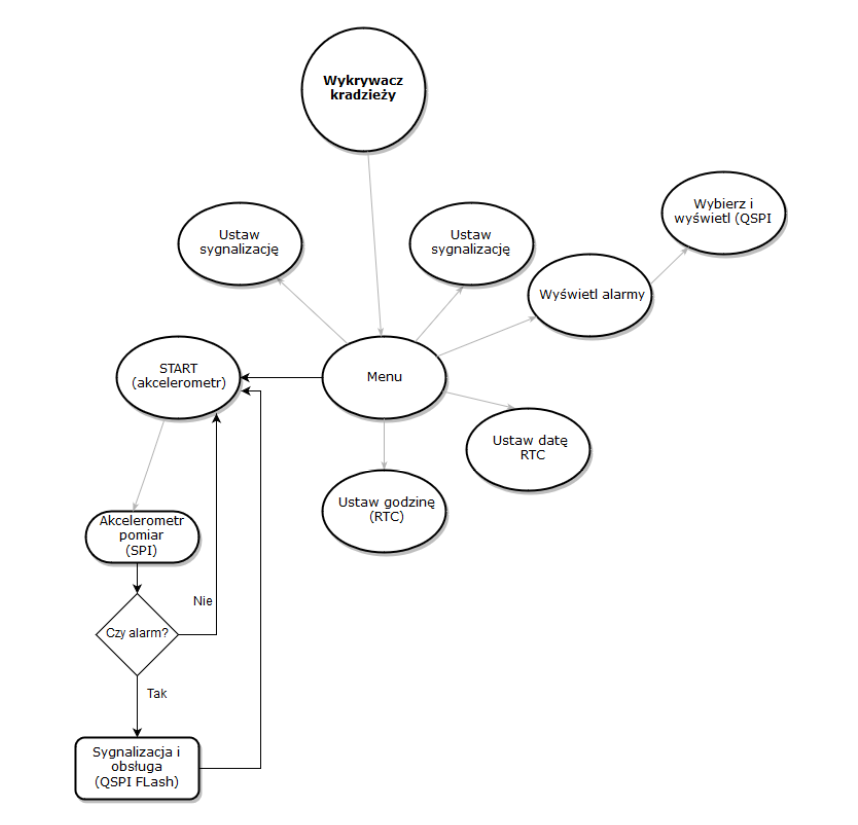
\includegraphics[width=13cm]{figures/d.png}
\caption{Schemat blokowy interakcji urządzenia z użytkownikiem}
\end{figure}
\section{Testowanie urządzenia}
Urządzenie testowano pod kątem dobrania odpowiedniej wartości przyspieszenia oznaczającego kradzież. Podczas oprogramowywania założono, że urządzenie -- podczas faktycznego używania w celu wykrycia kradzieży -- będzie znajdowało się w torebce lub plecaku użytkownika. W kontekście tego przeprowadzono testy symulujące upadek z $50cm$. \\ 
Jak widać na wykresie przy każdym upadku przyspieszenie najpierw spada do bardzo niskich wartości następnie rośnie. W większości przypadków nieznacznie w kontekście kolejnego wykresu, z symulacją kradzieży. Tylko jeden pomiar przekracza $100 \frac{m}{s}$ i jedynie kolejne 2 mają wartości na poziome $70 \frac{m}{s}$. Wszystkie pomiary stabilizują się w okolicach $16 \frac{m}{s}$. Pomiary te nie oddają w pełni upadku swobodnego, ze względu na to że płytka STM32L476 Discovery musi być podłączona do źródła zasilania kablem, który nieco ją blokuje.

\begin{figure}[H]
\centering
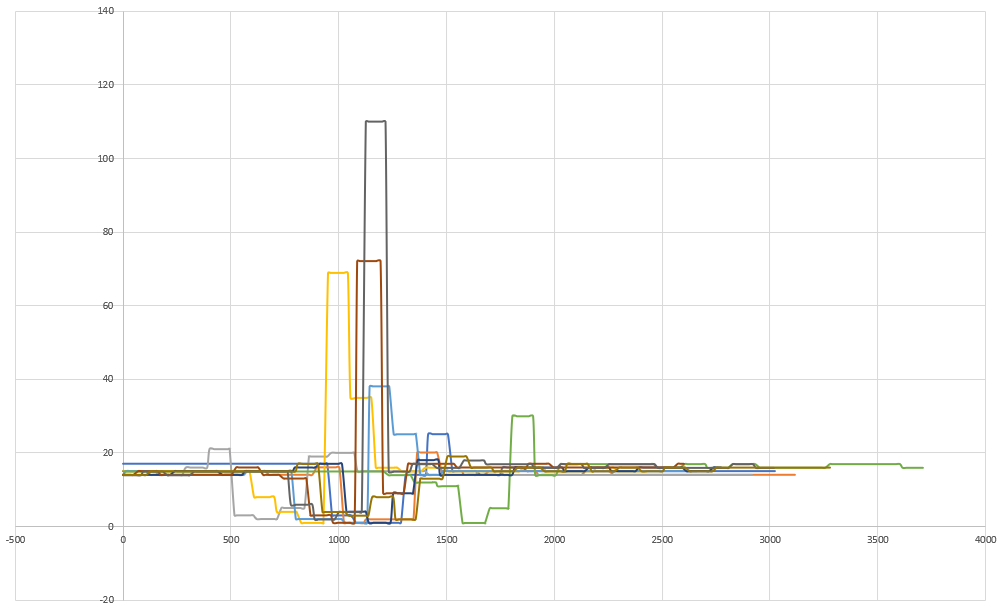
\includegraphics[width=13cm]{figures/t1.png}
\caption{Upadek z 50cm}
\end{figure}

Na kolejnym wykresie przedstawiono symulację poruszania się z torebką, w zwykły sposób. Pik, który można zaobserwować na wykresie, jest to zarzucenie torebki z urządzeniem na ramię. Jak widać tego typu zdarzenia nie powinny mieć wartości przyspieszenia większej od $100 \frac{m}{s}$. 
\begin{figure}[H]
\centering
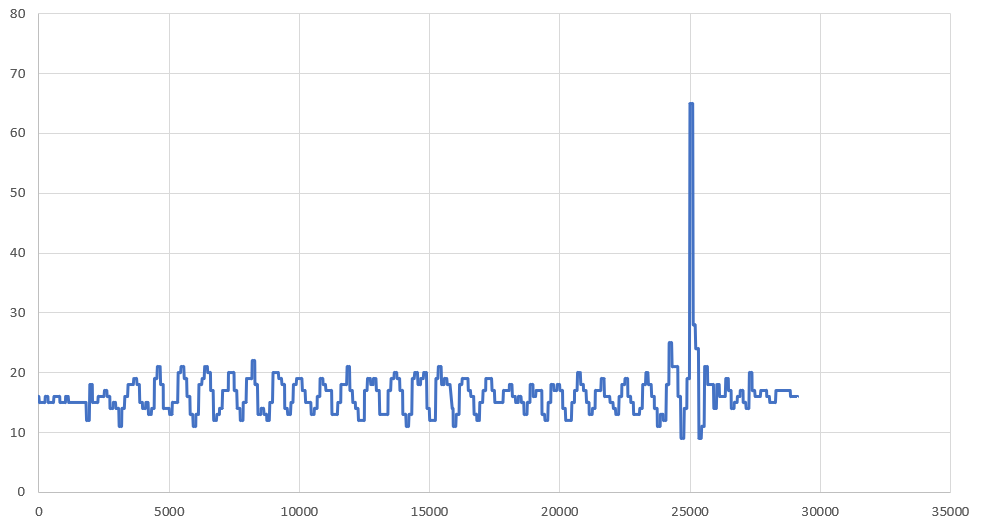
\includegraphics[width=13cm]{figures/t2.png}
\caption{Symulowane dopuszczalne przyspieszenia}
\end{figure}
Następy wykres przedstawia symulację kradzieży, zakładamy szarpanie kradniętym przedmiotem, następują częste bardzo wysokie piki wykrywanego przyspieszenia. Największe wartości oscylują wokół $130\frac{m}{s}$.  \begin{figure}[H]
\centering
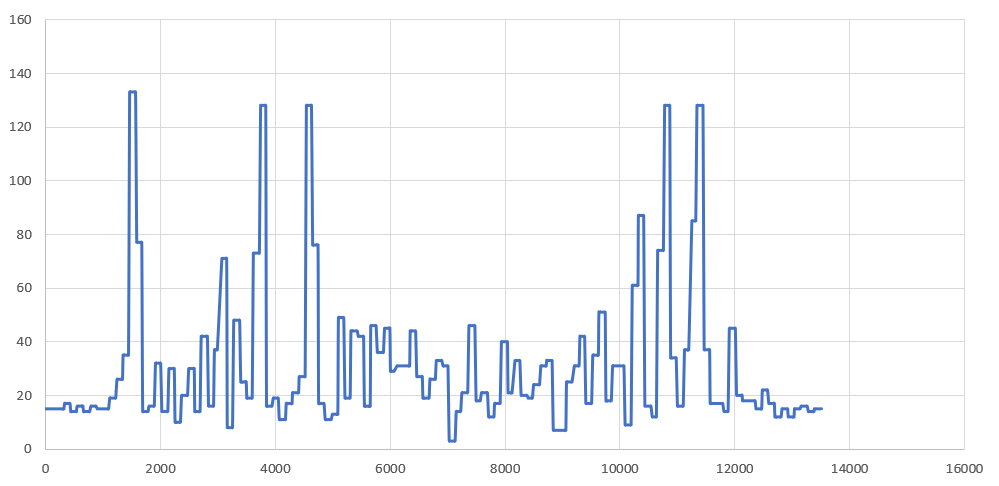
\includegraphics[width=13cm]{figures/t3.png}
\caption{Symulowana kradzież}
\end{figure}

%\section{Założenia projektowe}
%\begin{enumerate}
%\item Projekt będzie wykonywany w oparciu o płytkę STM32L476 Discovery wypożyczoną od prowadzącego kurs
%\item Pomiar przyspieszenia będzie odbywał się przez wbudowany moduł z akcelerometrem
%\item W przypadku wykrycia alarmu urządzenie podejmie określone kroki.
%\item Menu sterowane z joystick'iem zapewni możliwość wybór ustawień sygnalizacji alarmu(dioda oraz głośnik).
%\item Zbieranie danych o alarmach i przechowywanie w pamięci Flash.
%\item Wykorzystanie zegara RTC do umiejscowienia zdarzenia alarmu w jego lokalnym czasie.
%\item Badania dotyczące wykrywania progu alarmu i sprawdzenie funkcjonalności zaprojektowanego urządzenia.
%
%\end{enumerate}
%
%
%\section{Harmonogram pracy}
%
%\subsection{Zakres prac}
%Zapoznanie się z mikrokontrolerem, konfiguracja peryferiów. Implementacja obsługi zarówno pamięci Flash, jak i akcelerometru. Skonfigurowanie zegara RTC w celu późniejszej implementacji przekazywania godziny nieplanowanego ruchu. Zapoznanie z literaturą i poruszanym problemem. Przeprowadzenie badań na temat progów i optymalizacji działania urządzenia. 
%\subsection{Kamienie milowe}
%\begin{enumerate}
%\item Oddanie I etapu projektu. Projekt powinien zawierać założenia oraz plan co będzie podstawą do rozpoczęcia prac.
%\item Oddanie II etapu projektu. Konfiguracja peryferiów powinna być już sfinalizowana, a przynajmniej na etapie pozwalającym rozpoczęcie kolejnego etapu związanego z badaniem przyspieszeń które powinny aktywować alarm.
%\item Oddanie III etapu gdzie projekt powinien być już kompletny.
%Wg planu projekt powinien zakończyć się tydzień przed ostatecznym terminem złożenia pracy u prowadzącego.
%\end{enumerate}
%\subsection{Diagram Gantta}
%
%
%\begin{figure}[H]
%	\centering
%	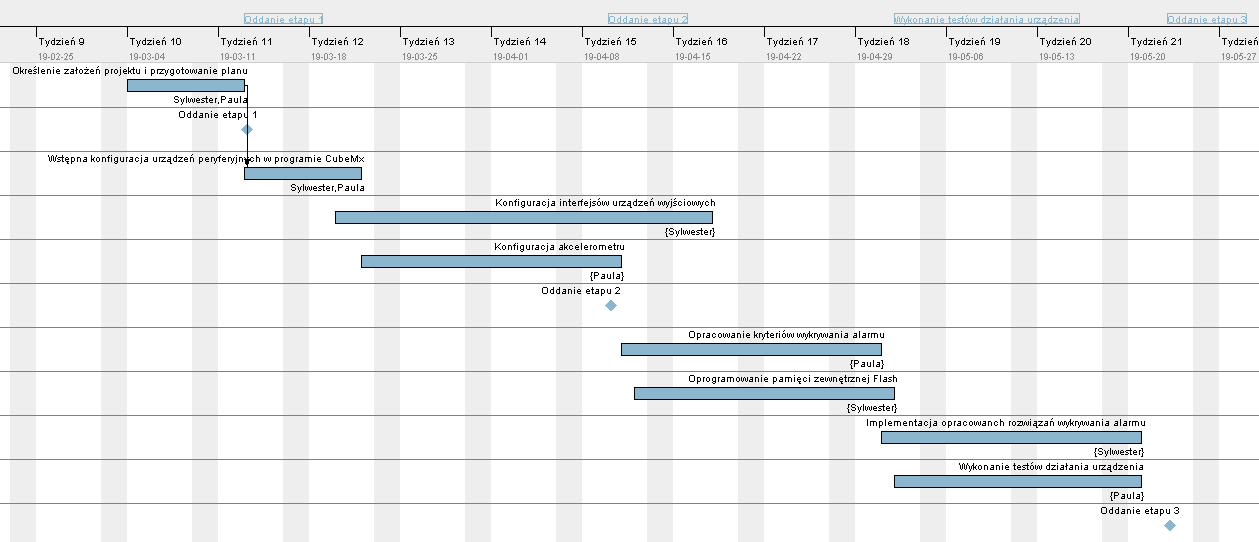
\includegraphics[width=1\textwidth]{figures/dg.png}
%	\caption{Diagram Gantta}
%	\label{fig:DiagramGantta}
%\end{figure}
%
%%Obecne w dokumencie do etapu I
%
%\subsection{Podział pracy}
%Oboje uczestnicy projektu zajmą się wstępną konfiguracją peryferiów odbywającą się za pomocą programu CubeMx. Zostanie zaimplementowana obsługa pamięci Flash, a także akcelerometru. W tym czasie opracowany zostanie również sposób przechowywania danych na zewnętrznej pamięci Flash. Projekt menu ma zakładać możliwość wyboru sygnału uruchamiającego alarm.
%
%\begin{table}[H]
%	\centering
%	\begin{tabular}{|L{7cm}|L{0.8cm}||L{7cm}|L{0.8cm}|}
%		\hline
%		\hline
%		\textbf{Sylwester Kozieja} & 
%		\% & 
%		\textbf{Paula Langkafel} & \%\\
%		\hline
%		\hline
%		Wstępna konfiguracja peryferiów w programie CubeMx		& &	
%		Wstępna konfiguracja peryferiów w programie CubeMx & \\
%		\hline
%		Wstępny projekt menu& &
%		Implementacja obsługi akcelerometru &\\
%		
%		\hline Konfiguracja zegara RTC & & &\\
%		\hline
%	\end{tabular}
%	\caption{Podział pracy -- Etap II}
%	\label{tab:PodzialPracyEtap2}
%\end{table}
%
%\begin{table}[H]
%	\centering
%	\begin{tabular}{|L{7cm}|L{0.8cm}||L{7cm}|L{0.8cm}|}
%		\hline
%		\hline
%		\textbf{Sylwester Kozieja} & 
%		\% & 
%		\textbf{Paula Langkafel} & \%\\
%		\hline
%		\hline
%		Oprogramowanie zewnętrznej pamięci Flash oraz opracowanie sposobu przechowywania danych		& &	
%		Opracowanie kryteriów wykrywania alarmu &\\
%		\hline
%		Implementacja opracowanych rozwiązań wykrywania alarmu  & &
%		Wykonanie testów urządzenia &\\
%		\hline
%		Sygnalizacja audiowizualna za pomocą Audio DAC oraz diody LED & & &\\
%		\hline
%	\end{tabular}
%	\caption{Podział pracy -- Etap III}
%	\label{tab:PodzialPracyEtap3}
%\end{table}

\section{Zakres wykonanej pracy}
\subsection{Akcelerometr}
Akcelerometr działa na komunikacji przez SPI, w trybie half duplex master. Piny dotyczące innych peryferiów w pewien sposób związanych z używanymi zostały wprowadzone w stan wysoki, tak żeby nie zakłócać pomiaru.
\subsection{Wyświetlacz z menu i zegarem RTC}
Pierwszy commit miał na celu stworzenie pierwszego prostego programu, który sprawdzał komunikację z diodami LED oraz wyświetlaczem.
W drugim commicie zostało zaimplementowane menu wraz z podstawowymi opcjami i zegar RTC będący podstawą do obliczania czasu co jest niezbędne do umiejscowienia alarmu w czasie. Urządzenie inicjowane jest stałą datą i godziną, ale istnieje możliwość ustawienia czasu w menu. Również w menu można ustawić flagi aktywność sygnalizacji alarmu dźwiękiem i diodą.



\subsection{Opis menu}

Opcje menu:
\begin {itemize}
\item Start - uruchamia procedurę rejestrowania alarmów
\item Ustaw godzinę
\item Ustaw datę
\item Audio - ustawienie sygnalizacji alarmu przez sygnał Audio
\item LED -ustawienie sygnalizacji alarmu diodą LED
\item Wyświetl alarmy - pobiera z pamięci zarejestrowane alarmy i wyświetla w postaci listy

\end {itemize}

\section{Podsumowanie}
Urządzenie może być wykorzystywane jako wykrywacz kradzieży, taka jest jego podstawowa funkcja. Ponadto przy włączeniu tylko jednej osi i zamontowaniu w samochodzie urządzenie może być wykorzystywane do na przykład oceny jakości dróg.  



%\section{Podsumowanie etapu III}
%\subsection{Akcelerometr}
%Akcelerometr został oprogramowany. 


\newpage
%\section{Literatura}
%\begin{enumerate}
%\item Vehicle Tracker wih a GPS and Accelerometer Sensor System in Jakarta - Suryadiputra Liawatimena, Jimmy Linggarjati
%\item UM1928 User manual - Getting started with STM32L476G discovery kit software development tools \\ \url{https://www.st.com/content/ccc/resource/technical/document/user_manual/c8/6c/20/e4/8c/3c/4d/13/DM00217936.pdf/files/DM00217936.pdf/jcr:content/translations/en.DM00217936.pdf}
%\item Quantitative Accelerated Life Testing of MEMS Accelerometers - Marius Bazu, Lucian Galateanu, Virgil Emil Ilian, Jerome Loicq, Serge Habraken,
%Jean-Paul Collette
%\item Overview of ST-LINK derivatives \\ \url{https://www.st.com/content/ccc/resource/technical/document/technical_note/group0/30/c8/1d/0f/15/62/46/ef/DM00290229/files/DM00290229.pdf/jcr:content/translations/en.DM00290229.pdf}
%\item 

%\end{enumerate}

\nocite{*}
\addcontentsline{toc}{section}{Bibilografia}
\bibliography{bibliografia}
\bibliographystyle{plabbrv}



\end{document}



